
% XXX muss vmtl eig in BAsics
% To evaluate the quality of the material parameters we need a possibility to investigate the material response caused by the definition of the material parameters. Then we can compare this results with the load parameters and evaluate the quality of the current material parameters. Thus we have to use a simulation program to analyse the material behaviour for every iteration of material parameter values during the optimisation process. We decided to use \name{Abaqus} as simulation software, because of the intern scripting tool. With the \name{Abaqus} scripting tool one can run python scripts directly in \name{Abaqus} (see chapter XX). With special \name{Abaqus} commands one can use \name{Abaqus} with the same opportunities as with the GUI. 
% XXXX

% Therefore we choose simple load cases, which are easy to recalculate. AS explained in the chpater XX about the mathematical problem formulation, we have to define a parameter which defines the quality of the mechanical responses calculated by \name{Abaqus} compared to the ones from the MD-simulation. Therefore we first have to define adequate mechanical measurements which represent best the mechanical behaviour and contain information about the material parameters. Hence the stress and strain measurements in all normal and shear directions are possible quantities. Depending on the load case the measurements with the most useful information may vary.



\chapter{Script setup} \label{chap: modelsAndMethods}

The remarks in \autoref{chap: basics} demonstrate the necessity of an easy and fast procedure to determine material parameters for materials modelled with \acrshort{md} simulations. Deformation tests in \acrshort{md} simulations provide information about the mechanical behaviour of the materials. The aim of the developed optimisation process is to find material parameters which best represent this behaviour.
In the following chapter we describe workflow of the optimisation script. First we have a closer look at the structure of the process. Then we introduce the required input data. At the end the implementation is explained. \\

In deformation tests performed with \acrshort{md} simulations the material behaviour during the loading process is recorded (see \autoref{sec: MDBasics}). Therefore stress and strain values in all directions at discrete simulation time steps are available. In the following stress and strain data, measured during a loading process, are referenced as load reactions. In \autoref{subsec:loadParameters} we present their structure in detail. To extract material parameters from these load reactions, a constitutive model is required, which describes the stress-strain relation of a material through a functional relation. The constitutive model, with its corresponding material parameters, used in this work is presented in \autoref{sec: MDBasics}. Therefore an evaluation of the material parameters found by the optimisation algorithm is possible. This is done with a \acrshort{fem} simulation as described in \autoref{sec: FEMBasics}. It returns the stress strain reactions from a material corresponding its prescribed material parameters, constitutive model and the loading process. Consequently, load reactions measured in \acrshort{md} simulations can be compared with the ones computed in \acrshort{fem}. To represent the mechanical behaviour measured in \acrshort{md} simulations best, a small difference between the load reactions is favourable. Since the material parameters define the load reactions from \acrshort{fem}, their quality is implicitly measured. In other words, we have to minimize the difference between the load reactions to find the best material parameters. We use the Nelder-Mead algorithm, introduced in \autoref{subsec: numericalOptimization}, to perform this optimisation. This numerical algorithm is capable to minimize the value of a scalar function by optimizing multiple parameters. Optimising all material parameters from our constitutive model is easily possible, while the scalar minimization function poses a challenge. Its function value defines the quality of the \acrlong{omp}. As explained before, we use the difference between the load reactions to define the \acrlong{omp} quality. Since we want to fit the whole loading process, the difference at all time steps should be taken into account. To achieve this, we design a procedure, explained in \autoref{sec: errorCalculation}, to summarize all these differences into one error value. However, some terms need to be introduced first. 

% The difference between the load reactions reveals implicit the \acrshort{mpv} quality, as 

% Simulating a loading process with \acrshort{fem} gives stress strain values  This simulation returns stress strain values resultin
% This load reactions should be represented through a constitutive model. 
% Through the optimisation 
% This load reactions should be matched as good as possible with the material parameter values found by the optimisation. To evaluate this the stress-strain curves governed by \acrshort{md} and the one described by the optimized \acrshort{mpv} is measured. The quality of the \acrshort{mpv} is better, if the . In our problem formulation we have now the optimisation of the material parameters controlled by the minimization of the difference between the mechanical responses. In the next step we need to define this difference between the mechanical behaviour more precisely. For the mathematical formulation only one single value is allowed for the problem formulation. For a detailed explanation we now introduce the used model, the load cases and load parameters.


    
% The difference between the stress-strain curvesimulation and the one from  \acrshort{fem} 
% As minimization value we have to define a value that represents the error of mechanical response of the material. Therefore we compare the material behaviour defined through the material parameters with the one from the load parameters.
% As explained in chapter XX we use \name{\name{Abaqus}} as simulation software and the \name{Abaqus} internal scripting tool for the code. 


\section{Input data} \label{sec: inputData}

% In this section we introduce the used model and the applied load cases. 
%  We use it as one representative part of an infinitely extended material which is modelled through \acrshort{pbc} (see \autoref{chap: basics}). By the usage of this simple geometry we anticipate short simulation times. During the optimisation process this property is important for a fast evaluation of the result quality.  However, it is easy to apply different loads on a cube. This is much easier at simple geometries where we can apply uniform stresses or strains. Additional, the mechanical responses in these load cases are qualitatively known, whereby a evaluation of the results is intuitive.
% In \autoref{subsec: loadCases} we define the used load cases. To achieve an easy implementation in the \name{Abaqus} scripting interface we keep them simple. 

% - used elements
% - apply boundary conditions (amplitude)
% - 


% NOCH MEHR ÜBER DAS MODEL

In the following sections the required input data are introduced. There are multiple types of input data which are processed at different places in the code. In order to ensure the traceability, clear definitions are required for every type of input. 

\subsection{Load cases and evaluated reactions}\label{subsec: loadCases}

A load case defines the direction in which a load acts. Since we want reproducible and easy cases, we only allow loading in normal and principal shear directions. We use the \name{Abaqus} plug-in EasyPBC to apply these loadings. For a consistent naming, we adopt the signatures from EasyPBC for the load cases, defined in \autoref{tab:LoadCaseMapping}.
To model a more complex loading situation, it is possible to apply different load cases one after another. For example, we can apply a normal strain in $xx$-direction followed by a shear strain in $xz$-direction. Nevertheless, in one load case only one direction is loaded to avoid mutual influence. The optimisation algorithm requires the load reactions without any constrains for every load case. Only \acrshort{pbc} are applied which are described in \autoref{sec: MDBasics}. After the application of a load case, we have to decide which material responses we use to compare with our load parameters. We have the possibility to read out the stresses and strains in all normal and shear directions (see \autoref{tab:evaluatedReactions}). The quantities we choose for the comparison are called \acrlong{er}.
For a high result quality of our material parameters, we try to choose \acrlong{er}s where we can extract the most information about our material behaviour. These measurements vary depending on the applied load case. In \autoref{fig:evaluationMeasurements} an exemplary load case E11 (green) with possible corresponding evaluated reactions (yellow) is depicted.

% \begin{table}[h!] 
% \centering
% \caption{Mapping of load directions to load cases}
% \label{tab:LoadCaseMapping}
% \renewcommand{\arraystretch}{1.1}
% \begin{tabular}{C{0.2\textwidth}C{0.15\textwidth}}
% \toprule
% \textbf{Load direction} & \textbf{Load case} \\ \midrule
% $xx$ & E11 \\ \hline
% $yy$ & E22 \\ \hline
% $zz$ & E33  \\ \hline
% $xy$ & G12 \\ \hline
% $yz$ & G23 \\ \hline
% $xz$ & G13 \\ \bottomrule
% \end{tabular}
% \end{table}

% \begin{table}[H]
% \centering
% \caption{list of possible evaluated reactions}
% \label{tab:evaluatedReactions}
% \renewcommand{\arraystretch}{1.1}
% \begin{tabular}{C{0.25\textwidth}C{0.25\textwidth}}
% \toprule
% \textbf{Evaluated stress reactions (ESR)} & \textbf{Evaluated strain reactions (EER)} \\ \midrule
% $\sigma_{xx}$ & $\varepsilon_{xx}$ \\ \hline
% $\sigma_{yy}$ & $\varepsilon_{yy}$  \\ \hline
% $\sigma_{zz}$ & $\varepsilon_{zz}$ \\ \hline
% $\sigma_{xy}$ & $\varepsilon_{xy}$ \\ \hline
% $\sigma_{yz}$ & $\varepsilon_{yz}$ \\ \hline
% $\sigma_{xz}$ & $\varepsilon_{xz}$ \\ \bottomrule
% \end{tabular}

% \end{table}

\begin{table}[h!]
\centering
\caption{Mapping of load directions and evaluated reactions}
\label{tab:CombinedOverview}
\renewcommand{\arraystretch}{1.0}

\begin{subtable}[t]{0.45\textwidth}
\centering
\caption{Mapping of load directions to load cases}
\label{tab:LoadCaseMapping}
\begin{tabular}{C{0.4\textwidth}C{0.3\textwidth}}
\toprule
\textbf{Load direction} & \textbf{Load case} \\ \midrule
$xx$ & E11 \\ \midrule
$yy$ & E22 \\ \midrule
$zz$ & E33 \\ \midrule
$xy$ & G12 \\ \midrule
$yz$ & G23 \\ \midrule
$xz$ & G13 \\ 
\bottomrule
\end{tabular}
\end{subtable}
\hfill
\begin{subtable}[t]{0.45\textwidth}
\centering
\caption{List of possible evaluated reactions}
\label{tab:evaluatedReactions}
\begin{tabular}{C{0.45\textwidth}C{0.45\textwidth}}
\toprule
\textbf{Evaluated stress reactions} & \textbf{Evaluated strain reactions} \\ \midrule
$\sigma_{xx}$ & $\varepsilon_{xx}$ \\ \midrule
$\sigma_{yy}$ & $\varepsilon_{yy}$ \\ \midrule
$\sigma_{zz}$ & $\varepsilon_{zz}$ \\ \midrule
$\sigma_{xy}$ & $\varepsilon_{xy}$ \\ \midrule
$\sigma_{yz}$ & $\varepsilon_{yz}$ \\ \midrule
$\sigma_{xz}$ & $\varepsilon_{xz}$ \\ 
\bottomrule
\end{tabular}
\end{subtable}

\end{table}


For the verification of the code we use a simple tensile load case E11.
In all other directions we impose no restrictions except \acrshort{pbc}. As \acrlong{er} we use $\sigma_{xx}$ and the lateral strains $\varepsilon_{yy}$ and $\varepsilon_{zz}$. The normal stress contains information about the Young's modulus and the plastic parameters. The lateral strains are necessary for the identification of the Poisson's ratio. Applying a strain in $xx$-direction will lead to decreasing dimensions in $yy$- and $zz$-direction. This reaction is necessary to keep a state of minimum stress. Simultaneously this means that the lateral stresses do not contain any useful information, because they are numerically zero. 
The validation study is realized with the same load case. Similar to the verification study we take $\sigma_{xx}$,  $\varepsilon_{yy}$ and $\varepsilon_{zz}$ to extract information about all material parameters. 
In the next step we handle load case E11, then G12 and finally combine them. Through the additional obtained information we try to improve the uniqueness of the determined material parameter values. As \acrlong{er} for the load case G12 we use the stresses $\sigma_{xy}$.
As a last study we investigate the application of cyclic loading as E11 load case. We perform this study with varying load parameters (see \autoref{subsec:loadParameters}). 


\begin{figure}[H]
    \centering
    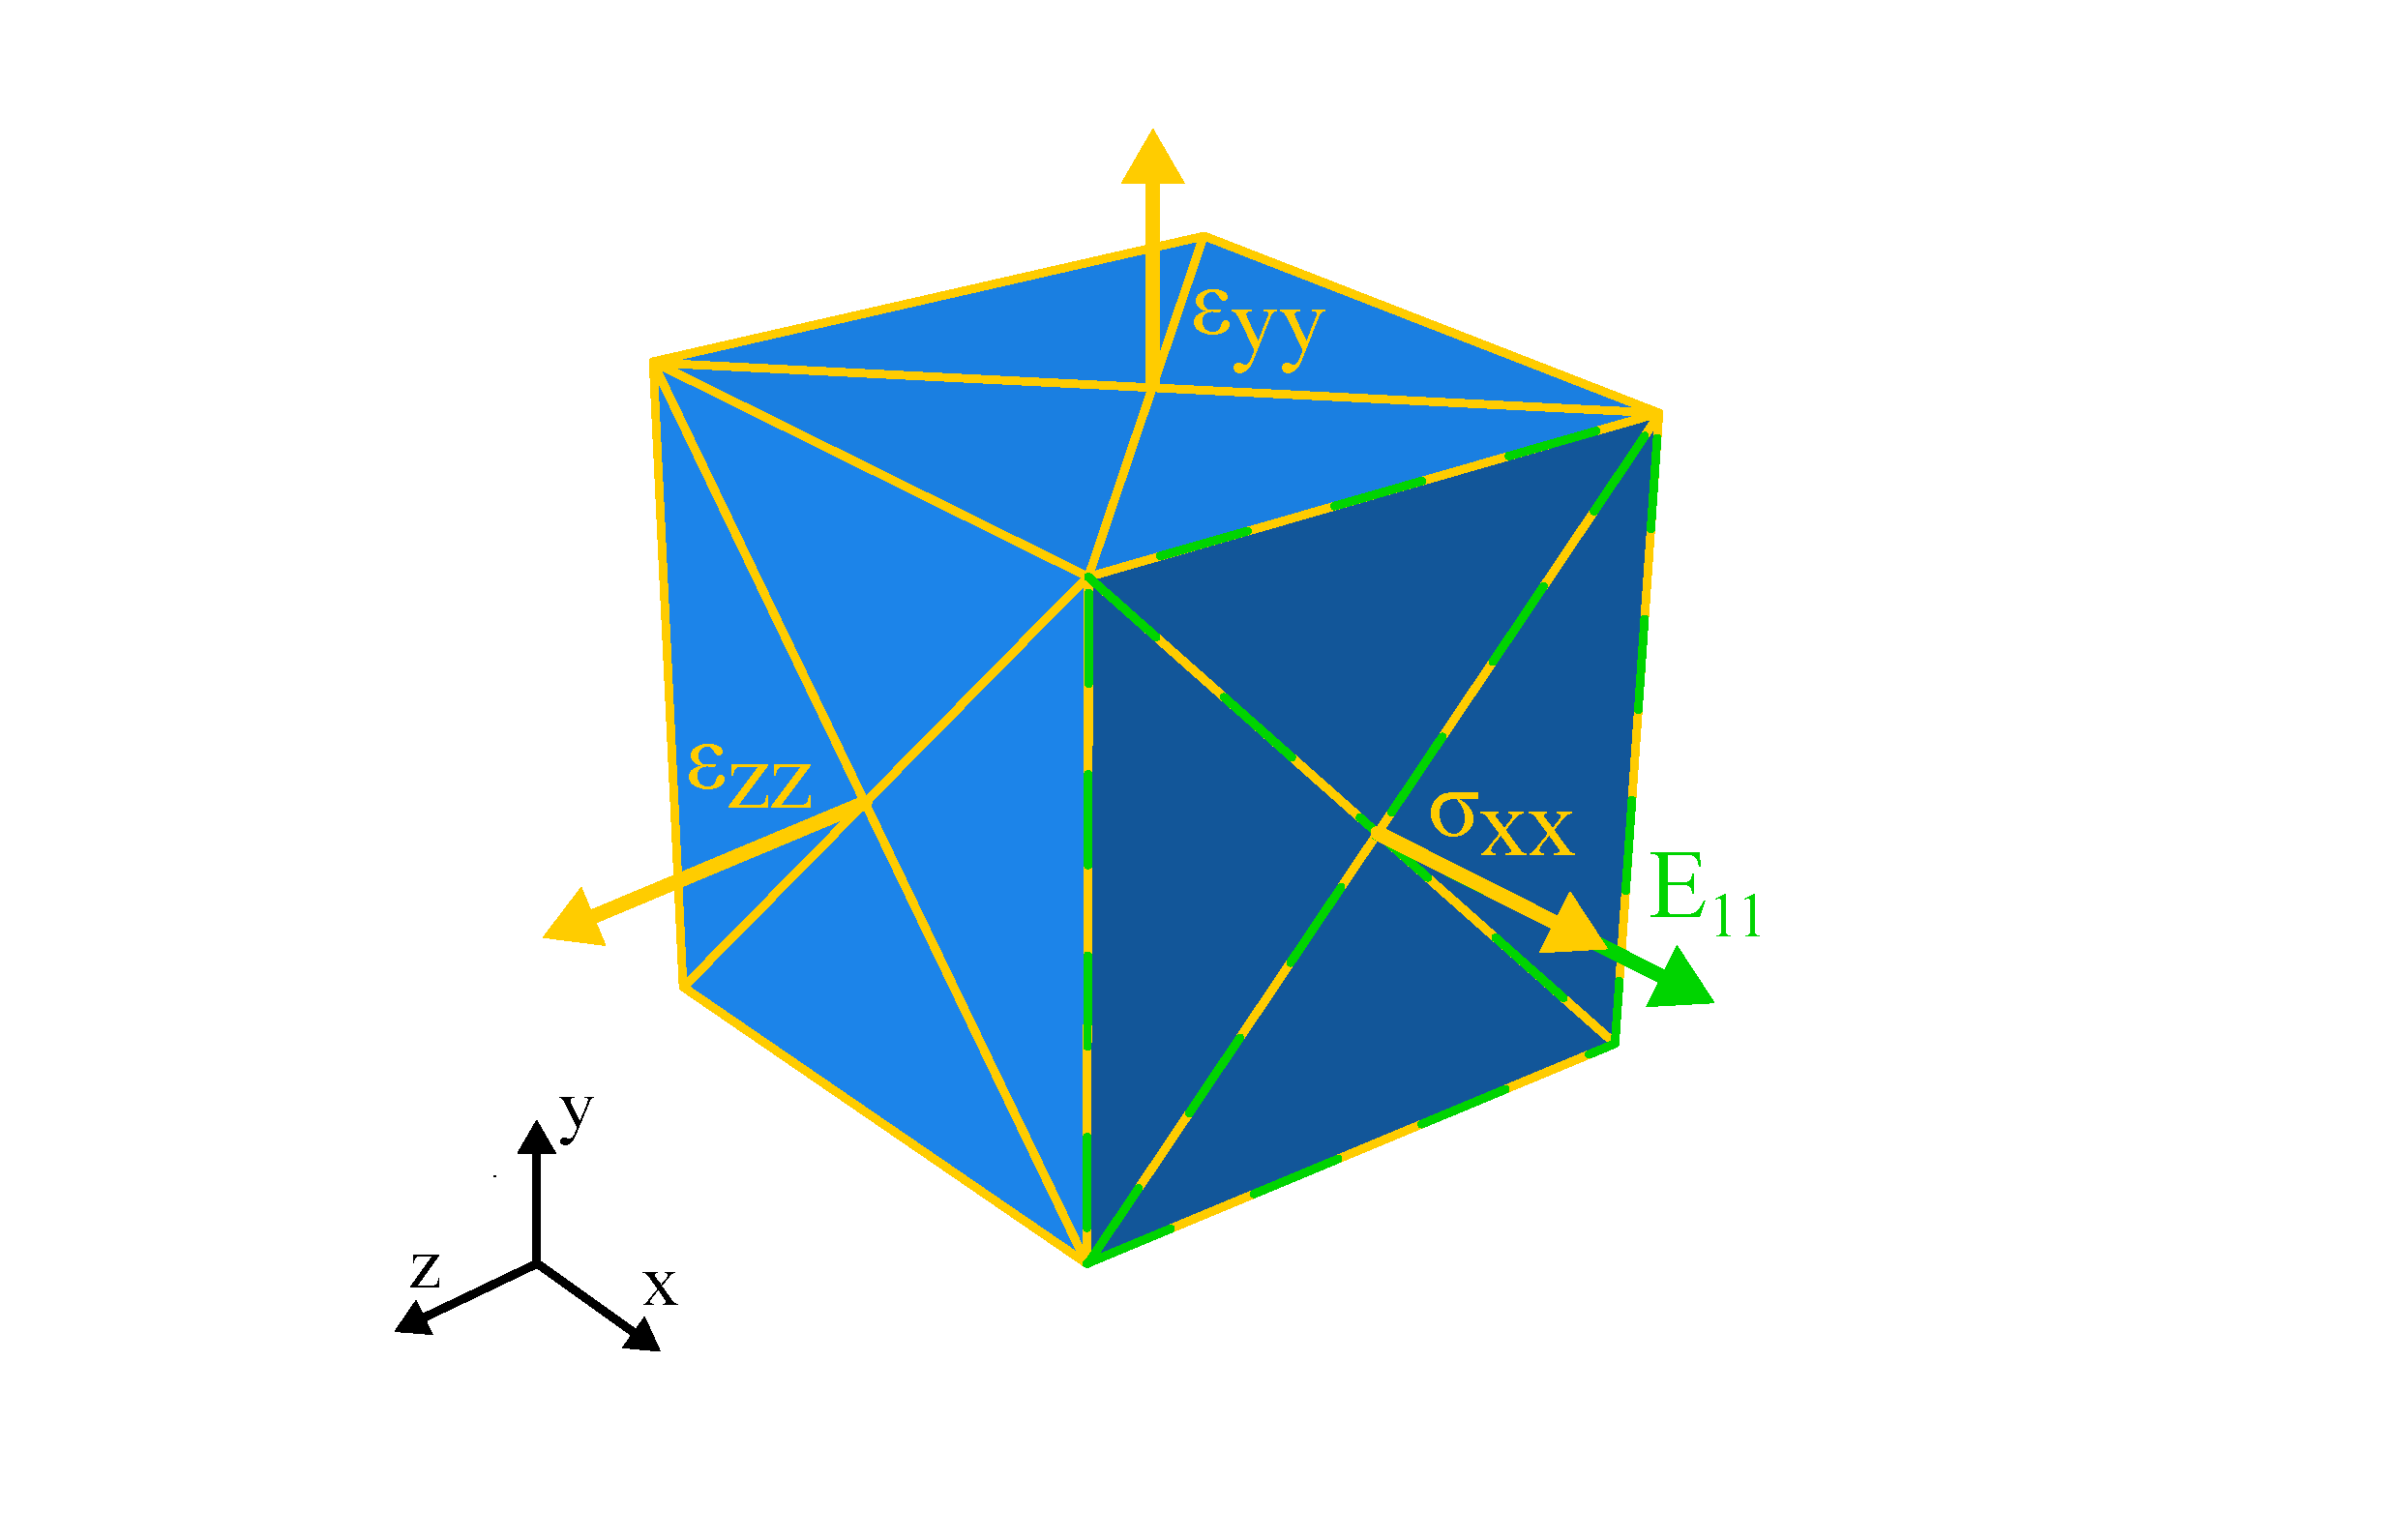
\includegraphics[width=0.7\textwidth]{cube_loading_plain_white_new.pdf}
    \caption{Illustration of load case E11 with its corresponding evaluated stress and strain reactions $\sigma_{xx}, \varepsilon_{yy}$ and $\varepsilon_{zz}$}
    \label{fig:evaluationMeasurements}
\end{figure}

\subsection{Load parameters and load reactions}\label{subsec:loadParameters}
For the optimisation process we use the data from \acrshort{md} simulations as input-file. This data are referenced as reference data in the following. They contain stress and strain values for all time steps during the loading process in all normal and shear directions. Thus, we can register different trends of loading with the corresponding responses.
We split the reference data into load parameters and \acrlong{rlr}. The load parameters define the quantitative values of the prescribed load case. 
Since we defined the load cases similar to the ones in the \acrshort{md} simulations, we can process the data from the load parameters directly.  If we know the load case, we can easily extract the load parameters from the reference data and transfer them into the \name{Abaqus} model. A detailed description of the load application in \name{Abaqus} can be found in \autoref{sec: preprocessing}. 
The \acrlong{rlr} represent the material response during the \acrshort{md} simulation. From this, we extract the stress and strain values according to the chosen \acrlong{er}. We neglect the remaining stress and strain values, since they probably contain little information about the material behaviour.
To perform the comparison of material behaviours we need analogous data from the \acrshort{fem} simulation. In the way described in \autoref{sec: optimizationCode} we can read out stress and strain values in all directions. Similar to the \acrlong{rlr} we extract the values corresponding to the \acrlong{er}. These values are called \acrlong{olr}. \\
\autoref{tab: testSeries} shows the investigated load cases and load parameters.
In the verification and validation studies we apply linear strain up to a maximum value of 20 \%. For the validation studies we use different mixing ratios which show different mechanical behaviours. Then we investigate a tensile strain following a sinus function over time with a maximum amplitude of 15 \% strain. We only consider the first quarter of one period up to the maximum value as a preparation for studies with cyclic loading. In this preparing study we want to investigate how non-linear loadings are handled. Then we use the same load parameters but apply them as shear strain. In the next step we use the same load parameters but combine the load cases of E11 and G12. Important to notice is that the previously introduced load parameters proceed in a wide strain range. Assuming that the material starts to plastify quite fast, the majority of the loading steps are located in the plastic domain of the material. Conversely, the load parameters contain only little information about the elastic material behaviour. In \autoref{sec: verification} the issue about this unequal distribution in the material domains becomes clear.    
As a last study we investigate  a full period of a sinusoidal loading for a tensile load case in $xx$-direction. We use amplitudes of 1 \%, 5 \% and 8 \%. Through the use of this load parameters we try to get a larger proportion of data points in the elastic domain.

\begin{table}[H]
    \centering
    \renewcommand{\arraystretch}{1.3}
    \caption{Overview of the performed tests with corresponding input parameters}
    \label{tab: testSeries}
    \begin{tabular}{L{0.17\textwidth}C{0.08\textwidth}C{0.13\textwidth}C{0.15\textwidth}C{0.13\textwidth}C{0.17\textwidth}}
    \toprule
    \multirow{2}{0.17\textwidth}{\textbf{Test series}} & \multirow{2}{0.08\textwidth}{\centering \textbf{Load case}} & \multicolumn{2}{C{0.28\textwidth}}{\textbf{\ Load parameters}} &  \multicolumn{1}{C{0.13\textwidth}}{\multirow{2}{0.13\textwidth}{\centering \textbf{Mixing ratio}}} &\multirow{2}{0.17\textwidth}{\centering \textbf{Evaluated reaction}} \\ \cmidrule{3-4}
    & &\textbf{Trajectory} & \textbf{Amplitude} & & \\  \midrule
    Verification & E11 & Linear & 20\% & 6:3 & \(\sigma_{xx}, \varepsilon_{yy}, \varepsilon_{zz}\)\\\hline
    Validation I & E11 & Linear & 20\% & 4:3 & \(\sigma_{xx}, \varepsilon_{yy}, \varepsilon_{zz}\)\\ \hline
    Validation II& E11 & Linear & 20\% & 6:3 & \(\sigma_{xx}, \varepsilon_{yy}, \varepsilon_{zz}\)\\ \hline
    Validation III& E11 & Linear & 20\% & 8:3 & \(\sigma_{xx}, \varepsilon_{yy}, \varepsilon_{zz}\)\\ \toprule
    \multirow{2}{0.15\textwidth}{Normal strain} & E11 & Sinus (\(\frac{1}{2} \pi\)) & 15\% & 6:3 & \(\sigma_{xx}, \varepsilon_{yy}, \varepsilon_{zz}\)\\ 
            &   &           &   && \\ \hline
    Shear strain  & G12 & Sinus (\(\frac{1}{2}\pi\)) & 15\% & 6:3 & \(\sigma_{xy}\)\\ \hline
    \multirow{2}{0.15\textwidth}{Normal \& Shear strain} & E11 & Sinus (\(\frac{1}{2}\pi\)) & 15\% & 6:3 & \(\sigma_{xx}, \varepsilon_{yy}, \varepsilon_{zz}, \sigma_{xy}\)\\ 
                            & G12 &       &      &     \\ \hline
    \multirow{2}{0.15\textwidth}{Normal strain} & E11 & Sinus (\(2\pi\)) & 1\%  & 6:3 & \(\sigma_{xx}, \varepsilon_{yy}, \varepsilon_{zz}\)\\ 
                &     &       & 5\%  &  & \(\sigma_{xx}, \varepsilon_{yy}, \varepsilon_{zz}\)\\ 
                &     &       & 8\%  & & \(\sigma_{xx}, \varepsilon_{yy}, \varepsilon_{zz}\)\\ \bottomrule
    \end{tabular}
    
\end{table}



\section{Error calculation}\label{sec: errorCalculation}
For a representative value including all necessary data we use the \acrshort{rmse}, which is explained in \autoref{subsec: RMSE}. Therefore, we use \autoref{eq: multiRMSE}, and include the data sets with the load reactions.
First we extract the \acrlong{rlr} and the \acrlong{olr} in the way described in \autoref{sec: optimizationCode}. In the next step we have to build the difference between them. We compute the difference between the load reactions at one load step and then iterate over all load steps. \autoref{fig: erroPlot} displays this procedure for an exemplary set of \acrlong{rlr} and \acrlong{olr}. Here $\sigma_{xx}$ is the selected \acrlong{er}. For every load step $\text{LS}_i$ their corresponding \acrfull{rlr} $\sigma_{\scriptscriptstyle\text{LS}_i}^{\scriptscriptstyle\text{RLR}}$ and \acrfull{olr} $\sigma_{\scriptscriptstyle\text{LS}_i}^{\scriptscriptstyle\text{OLR}}$ is logged. The blue arrow highlights their difference $\Delta\sigma_{\scriptscriptstyle\text{LS}_i}$ for one exemplary load step, according to \autoref{eq: EMDifference}. We square each of these differences to avoid negative values.  As described in \autoref{subsec:loadParameters}, the distribution of the data points is unfavourable for the determination of the elastic parameters. To support the algorithm to find the elastic parameters anyway, we applied a weight of 100 at the data point in the elastic domain. This is done via an array $\boldsymbol{w}$ which entries are one except the first entry $w_{\scriptscriptstyle\text{LS}_1}$. 
In the next step we build the mean value of the weighted arrays. The resulting value is called \acrfull{mse}. We compute the \acrshort{mse} for one \acrlong{er} according to \autoref{eq: mse}. We compute $\text{mse}_{\sigma}$ or $\text{mse}_{\varepsilon}$ for every selected \acrlong{er}. 

\begin{figure}[H]
    \centering
    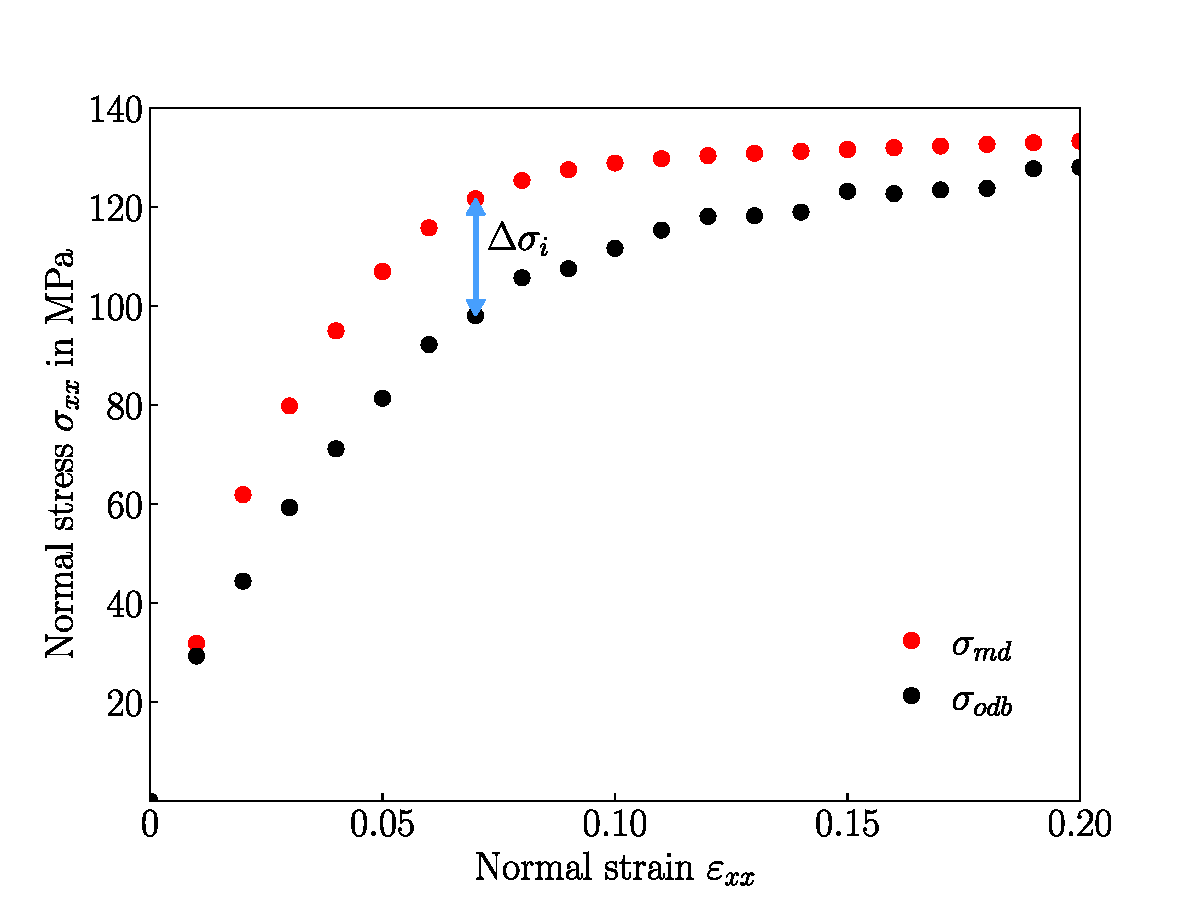
\includegraphics[width = 0.65\textwidth]{error_plot.pdf}
    \caption{Exemplary \acrlong{rlr} $\sigma^{\scriptscriptstyle\text{RLR}}$ and \acrlong{olr} $\sigma^{\scriptscriptstyle\text{OLR}}$ with visualization of error calculation}
    \label{fig: erroPlot}
\end{figure}


\begin{gather}
    \label{eq: EMDifference}
    \Delta\sigma_{\scriptscriptstyle\text{LS}_i} = \sigma_{\scriptscriptstyle\text{LS}_i}^{\scriptscriptstyle\text{RLR}} - \sigma_{\scriptscriptstyle\text{LS}_i}^{\scriptscriptstyle\text{OLR}} \hspace{2cm}
    \Delta\varepsilon_{\scriptscriptstyle\text{LS}_i} = \varepsilon_{\scriptscriptstyle\text{LS}_i}^{\scriptscriptstyle\text{RLR}} - \varepsilon_{\scriptscriptstyle\text{LS}_i}^{\scriptscriptstyle\text{OLR}}\\
    \label{eq: mse}
    \text{MSE}_{\sigma} = \frac{\displaystyle\sum_{\text{LS}} w_{\scriptscriptstyle\text{LS}} (\Delta\sigma_{\scriptscriptstyle\text{LS}}^2)}{\displaystyle\sum_{\text{LS}}w_{\scriptscriptstyle\text{LS}} } \hspace{2cm}
    \text{MSE}_{\varepsilon} = \frac{\displaystyle\sum_{\text{LS}} w_{\scriptscriptstyle\text{LS}} (\Delta\varepsilon_{\scriptscriptstyle\text{LS}})^2}{\displaystyle\sum_{\text{LS}}w_{\scriptscriptstyle\text{LS}}}
\end{gather}


% \begin{equation*}
%     N_{\text{LS}}: \text{Number of load steps}
%     \hspace{1.5cm}
%     w_i : \text{weight}
% \end{equation*}

For the tensile load case for example we must perform this for the \acrlong{er} $\sigma_{xx}, \varepsilon_{yy} \text{ and } \varepsilon_{zz}$. 
If we now construct a single value out of these \acrshort{mse}s we must ensure a common scale. Otherwise, their influence on the overall error may vary significantly. In general, the \acrshort{mse}s of \acrlong{eer} are much smaller than the ones from \acrlong{esr}, such that loading dependent weights $w_{\sigma}$ and $w_{\varepsilon}$ are introduced. The exact weights depend on the load case and the used load parameter set. In general, the \acrshort{mse}s of \acrlong{eer} are much smaller than the ones from \acrlong{esr}, such that a weight $w_{\varepsilon}$ of around $10^4$ is necessary for $\text{mse}_{\varepsilon}$. After that we sum up the weighted \acrshort{mse} and construct the \acrshort{rmse} as shown in \autoref{eq: rmse}. Since our code is able to process multiple load cases in one optimisation process we can calculate the \acrshort{rmse} for every load case and apply weights $w_{\scriptscriptstyle\text{LC}}$ depending on the load case. Then we sum up all these weighted \acrshort{rmse} values. Additionally, multiple load parameters sets can be processed which leads to a repetition of the described procedure for every load parameter set. Then we can apply weights $w_{\scriptscriptstyle\text{LP}}$ for every load parameter set and sum it again, which results in a double sum according to \autoref{eq: error}. This value is the one we return our minimization function. In the following sections we have a closer look at the implementation of this minimization process. 

\begin{gather}
    \label{eq: rmse}
        \text{RMSE} = \sqrt{\frac{\displaystyle\sum_{\text{ESR}} w_{\sigma} \cdot \text{MSE}_{\sigma} + \displaystyle\sum_{\text{EER}} w_{\varepsilon} \cdot \text{MSE}_{\varepsilon}}{N_\text{ESR} + N_\text{EER}}} \\
        \label{eq: error}
    \text{Error} = \sum_{\text{LP}} \sum_{\text{LC}} w_{\scriptscriptstyle\text{LP}} w_{\scriptscriptstyle\text{LC}} \cdot \text{RMSE}_{\scriptscriptstyle \text{LC}, \text{LP}}
\end{gather}
\begin{gather*}
        N_\text{ESR}: \text{Number of \acrlong{esr}} \\
    N_\text{EER}: \text{Number of \acrlong{eer}}
\end{gather*}




\section{Preprocessing} \label{sec: preprocessing}


\begin{table}[H]
    \centering
    \caption{Input parameters for optimisation process}
    \label{tab: inputParameterTable}
    \renewcommand{\arraystretch}{1.1}
    \begin{tabular}{L{0.2\textwidth}C{0.2\textwidth}C{0.15\textwidth}C{0.1\textwidth}C{0.1\textwidth}}
    \toprule
    \textbf{Input parameter} & \textbf{Directions} & \textbf{Category} & \textbf{Data format} & \textbf{Unit} \\ \midrule
    Young's modulus & – & value    & array  & MPa \\ 
                & – & minimum  & scalar & MPa \\ 
                & – & maximum  & scalar & MPa \\ \hline
    Poisson's ratio  & – & value    & array  & –   \\ 
                & – & minimum  & scalar & –   \\ 
                & – & maximum  & scalar & –   \\ \hline
    Plastic Yield  & – & value    & array  & MPa \\ 
                & – & minimum  & scalar & MPa \\ 
                & – & maximum  & scalar & MPa \\ \hline
    \multirow{2}{0.2\textwidth}{Alpha, beta, gamma} & – & value    & array  & –   \\ 
                    & – & minimum  & scalar & –   \\ 
                    & – & maximum  & scalar & –   \\ \hline
    Load parameters & – & filename & string & –   \\ 
                    & – & weight   & scalar & –   \\ \hline
    Load case & \multirow{2}{0.2\textwidth}{E11, E22, E33, G12, G23, G13} & active & boolean    & – \\ 
            &                               & weight & scalar & – \\ \hline
    Stress evaluation & \multirow{2}{0.15\textwidth}{$xx$, $yy$, $zz$, $xy$, $yz$, $xz$} & active & boolean   & – \\ 
                    &                        & weight & scalar & – \\ \hline
    Strain evaluation & \multirow{2}{0.15\textwidth}{$xx$, $yy$, $zz$, $xy$, $yz$, $xz$} & active & boolean  & – \\ 
                    &                        & weight & scalar & – \\ \hline
    Load weighting & \multirow{4}{0.2\textwidth}{normal stress, normal strain, shear stress, shear strain} & weight & scalar & – \\ 
    &&&& \\
    &&&& \\
    &&&& \\\bottomrule
    \end{tabular}
    
\end{table}


Before starting with the optimisation process, we need preprocessing steps to create a working \name{Abaqus} model with the required properties. In \autoref{fig: flowchart} the complete structure of the code is depicted. The white boxes show the individual steps referred to in the text in italics. The coloured boxes represent the performed loops. The upper part belongs to the preprocessing, which start with the step \benennung{Read input file}. \autoref{tab: inputParameterTable} lists an extract of this file containing only parameters relevant for the optimisation process. The input file contains more parameters for different namings, which are neglected here. In attaachment XX the whole input file is included. The user has multiple options to specify the optimisation process. It is possible to test multiple initial value combinations for the material parameters calling the script once. In \autoref{tab: inputParameterTable} this is visible in the column \benennung{Data format} of the values of all material parameters. This function is important, to verify the optimisation results with varying input values. For every material parameter we write an array of initial values. Then the code loops over all array entries at a time to extract one initial value for each parameter. Therefore, the entries with the same index add up to one initial value combination which is visualized in \autoref{tab:material_combinations}. As a consequence all arrays need to be of same length. For all initial value combinations the code creates a new \acrfull{mdb} in \name{Abaqus}, and a new folder structure to set the working directory and store the results.




\begin{table}[h!]
    \centering
    \caption{Loop conditions in preprocessing}
    \label{tab:loop_conditions}
    \begin{subtable}[t]{0.45\textwidth}
        \centering
        \renewcommand{\arraystretch}{1.1}
        \caption{Arrangement of initial value combination of material parameters}
        \label{tab:material_combinations}
        \begin{tabular}{L{0.31\textwidth}|C{0.08\textwidth}C{0.08\textwidth}C{0.08\textwidth}C{0.08\textwidth}C{0.08\textwidth}}
            \toprule
            \multirow{2}{0.31\textwidth}{\textbf{Material Parameter}} & \multicolumn{5}{c}{\textbf{Combination}} \\
            \cmidrule(lr){2-6}
             & \textbf{1} & \textbf{2} & \textbf{3} & \textbf{4} & \textbf{5} \\ \midrule
            $E$ & $E_1$ & $E_2$ & $E_3$ & $E_4$ & $E_5$ \\ \hline
            $\nu$ & $\nu_1$ & $\nu_2$ & $\nu_3$ & $\nu_4$ & $\nu_5$ \\\hline
            $\sigma_{\mathrm{pl}}$ & $\sigma_{\mathrm{pl1}}$ & $\sigma_{\mathrm{pl2}}$ & $\sigma_{\mathrm{pl3}}$ & $\sigma_{\mathrm{pl4}}$ & $\sigma_{\mathrm{pl5}}$ \\\hline
            $\alpha$ & $\alpha_1$ & $\alpha_2$ & $\alpha_3$ & $\alpha_4$ & $\alpha_5$ \\\hline
            $\beta$ & $\beta_1$ & $\beta_2$ & $\beta_3$ & $\beta_4$ & $\beta_5$ \\\hline
            $\gamma$ & $\gamma_1$ & $\gamma_2$ & $\gamma_3$ & $\gamma_4$ & $\gamma_5$ \\ 
            \bottomrule
        \end{tabular}
    \end{subtable}  
    \hfill
    \begin{subtable}[t]{0.45\textwidth}
        \centering
        \renewcommand{\arraystretch}{1.1}
        \caption{Model creation for load case and parameter combinations}
        \label{tab:model_creation}
        \begin{tabular}{L{0.25\textwidth}|C{0.2\textwidth}C{0.35\textwidth}}
            \toprule
            \multirow{2}{0.25\textwidth}{\textbf{Model}} & \multirow{2}{0.2\textwidth}{\centering \textbf{Load case}} & \multirow{2}{0.35\textwidth}{\centering \textbf{Load parameters}} \\ 
            & & \\ \midrule
            Model 0 & E11 & Data set 1 \\ \hline
            Model 1 & E11 & Data set 2 \\\hline
            Model 2 & E11 & Data set 3 \\\hline
            Model 3 & G12 & Data set 1 \\\hline
            Model 4 & G12 & Data set 2 \\\hline
            Model 5 & G12 & Data set 3 \\
            \bottomrule
        \end{tabular}
    \end{subtable}    
\end{table}

FORMATIEREN


Afterwards we start the first loop with \benennung{Create model}. As discussed in \autoref{sec: FEMBasics} we model a cube with size 1x1x1. We mesh the cube with 6x6x6 elements. Because of the regular geometry, we work with hexagonal structured elements to keep the model simple. The number of elements is a compromise between a coarse mesh for fast computation and a minimum number to avoid convergence errors. Although we use a hyperelastic material in our optimisation process, we first have to build the model with elastic material. We apply isotropic behaviour and define Young's modulus and Poisson ratio as the initial values. The elastic material is necessary due to the usage of EasyPBC in the step \benennung{Create job}. We use the load case defined in the input file to create a job. As discussed in \autoref{subsec: EasPBC}, we use EasyPBC for the automatic construction of \acrshort{pbc}. Aside from that, we adopt the generated load application corresponding to the load case. Since the load acts on a reference point, connected to the whole loaded surface, a homogeneous load contribution is ensured.
However, the settings from EasyPBC contain some default values, we adjust in the step \benennung{Modify properties}. EasyPBC applies for every load case a uniform displacement with a standard fixed value, while we want to study the complete loading process. For a correct comparison of the loading reactions we have to evaluate the stresses and strains in the \acrshort{fem} simulation at the same step sizes as in the \acrshort{md} simulation. In \name{Abaqus} we can solve this issue by creating an amplitude to apply the load gradually (see \autoref{fig:amplitudemenu}). Therefore, we enter the load parameters as an amplitude at certain time steps. For the time steps we use consecutive numbers, since the steps sizes are already defined through the amplitude. The value in the boundary condition editor is then set to one because this only defines the factor by which the amplitude is multiplied (see \autoref{fig:bcmenu}). Afterwards we modify the increment settings. EasyPBC automatically creates increments with fixed size and without non-linear geometry effects. In order to avoid convergence errors, we use automatic incrementation. Especially in the first load steps, we observe large deformations. If we try to resolve such large deformations in one incrementation step, \name{Abaqus} runs into convergence errors. With automatic incrementation \name{Abaqus} can adapt the number of increments per load step dynamically dependent of the current deformation. The non-linear geometry effects have to be considered for the same reason. In the last step of preprocessing we store the model in a dictionary. We use this dictionary later to call the models for the optimisation. We perform the preprocessing for all prescribed load cases, highlighted in green in the flowchart. Furthermore, the purple area visualizes the loop over the load parameters. This leads to individual models for every load case and every load parameter set, which is visualized in \autoref{tab:model_creation}.

    \begin{figure}[H]
    \centering
    \begin{minipage}[T!]{1.0\textwidth}
        \centering
        \begin{minipage}[T!][9cm][T!]{0.35\textwidth}
            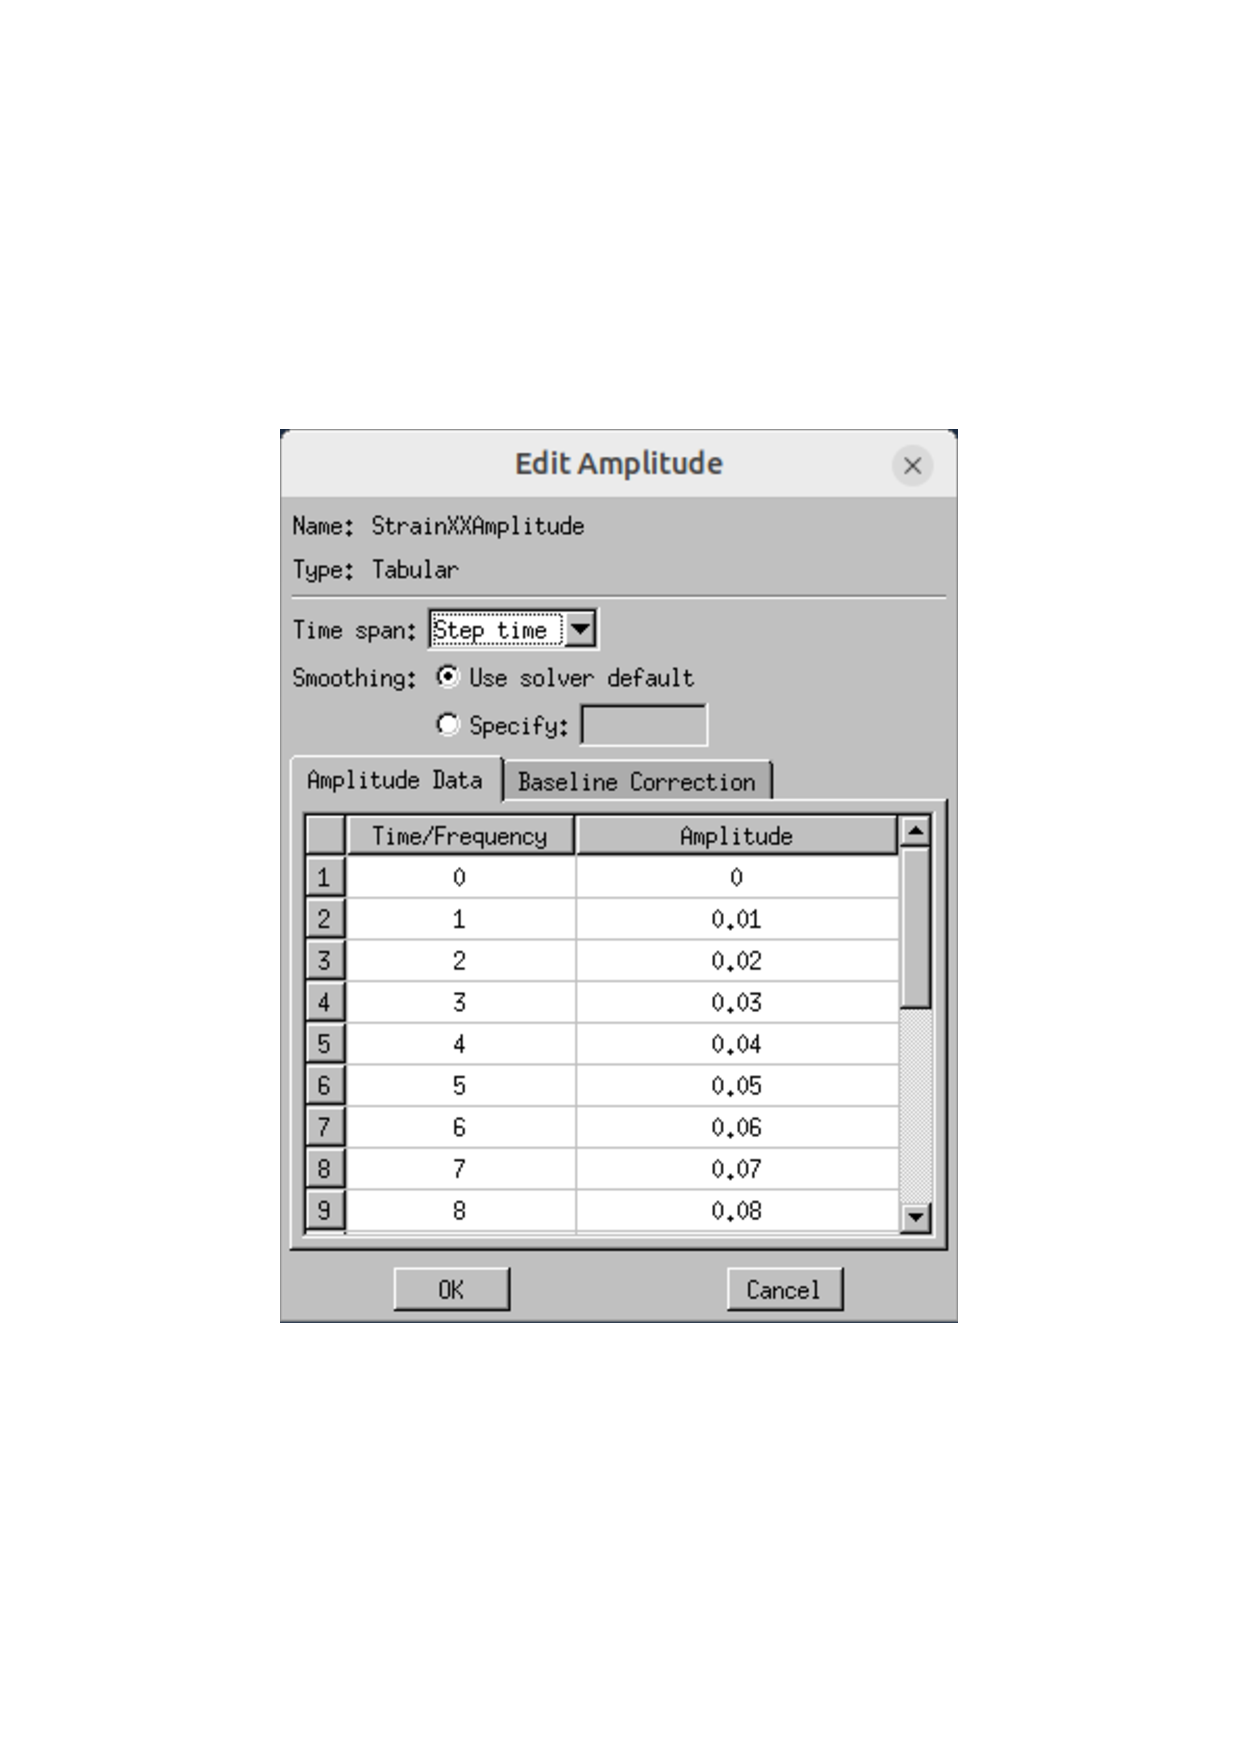
\includegraphics[width=1.0\textwidth]{Amplitude.pdf}
            \vfill{}
            \caption*{(a) Definition of load amplitude in \name{Abaqus}}
            \label{fig:amplitudemenu}
        \end{minipage}
        \hspace{0.08\textwidth} % Horizontal space between the minipage
        \begin{minipage}[T!][9cm][T!]{0.35\textwidth}
            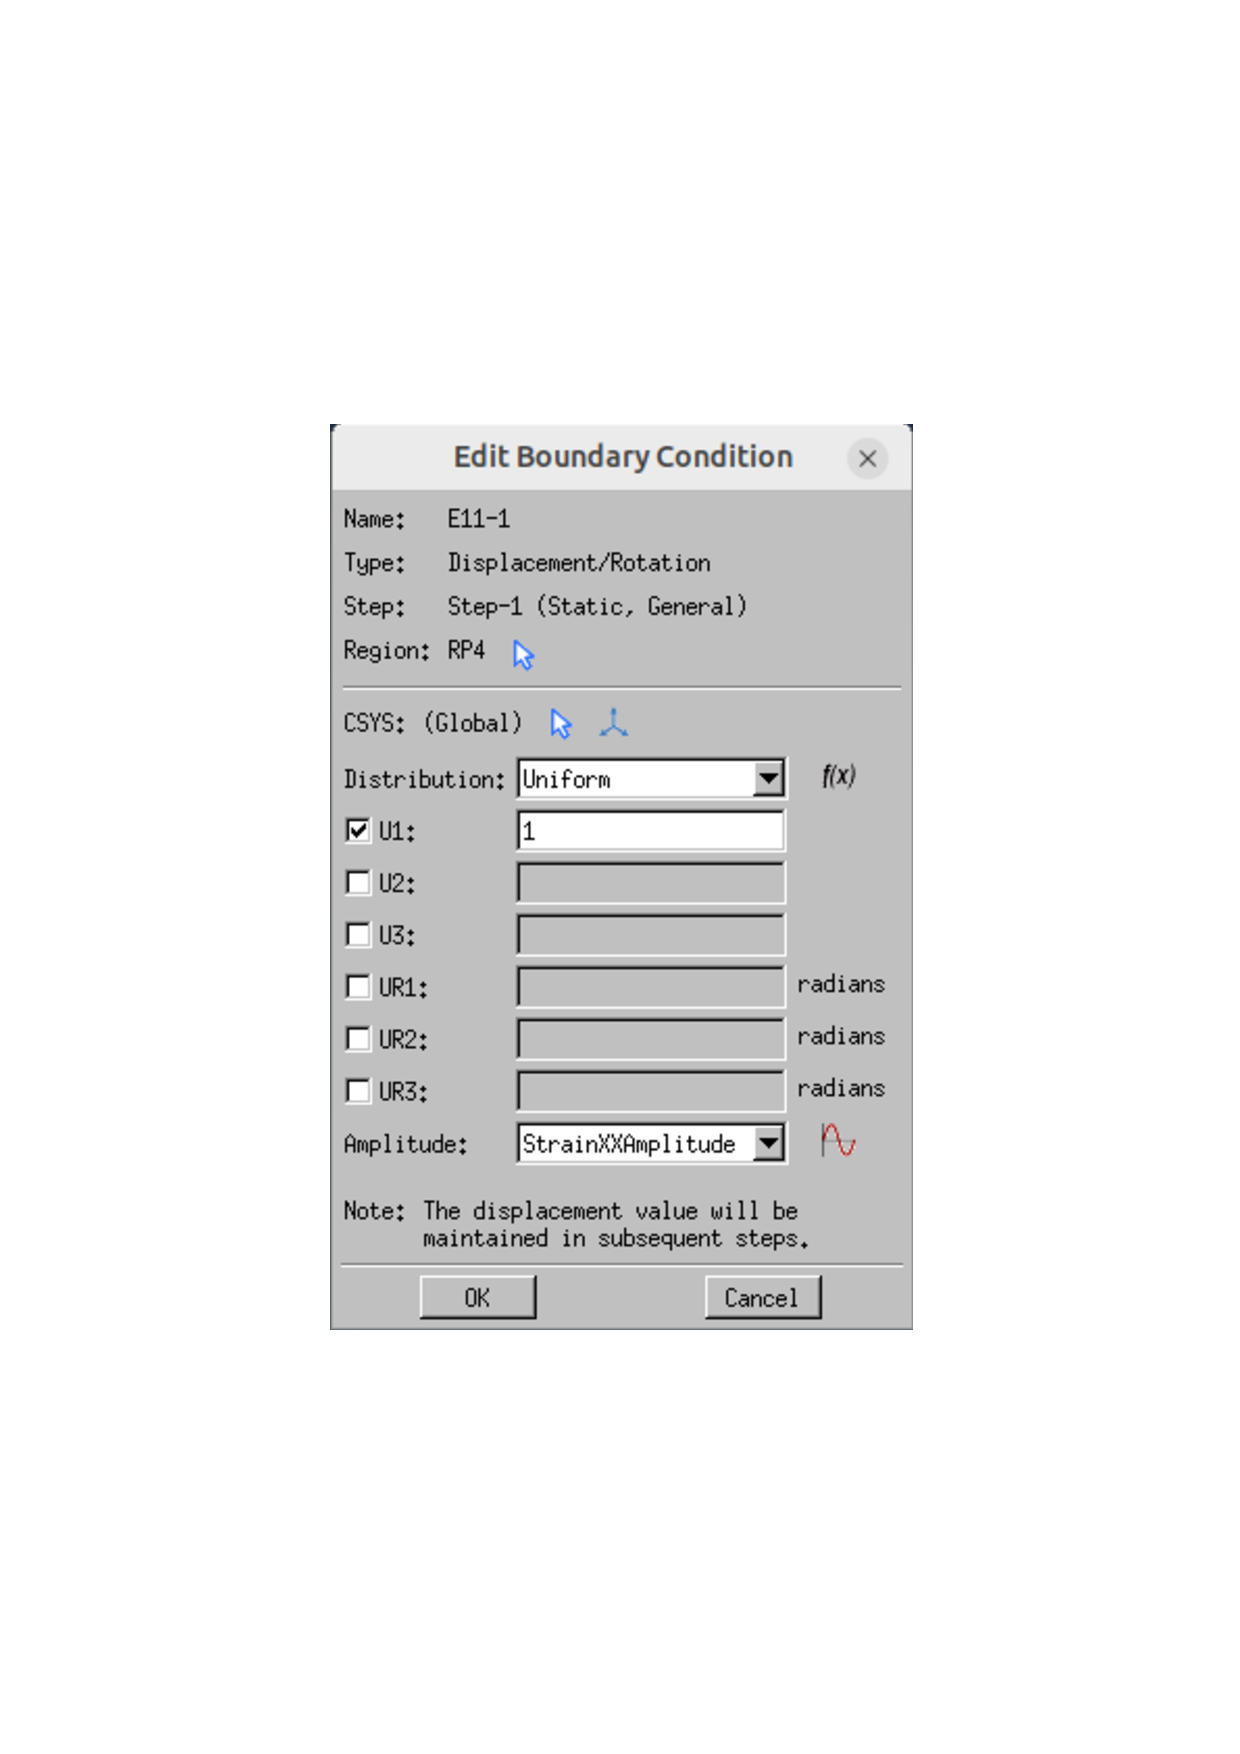
\includegraphics[width=1.0\textwidth]{BC.pdf}
            \vfill{}
            \caption{Boundary condition menu in \name{Abaqus}}
            \label{fig:bcmenu}
        \end{minipage}
    \end{minipage}    
    \caption{Loop conditions in preprocessing}
    \label{fig:Abaqus Settings}
\end{figure}

\section{Optimisation process} \label{sec: optimizationCode}

\begin{figure}[H]
    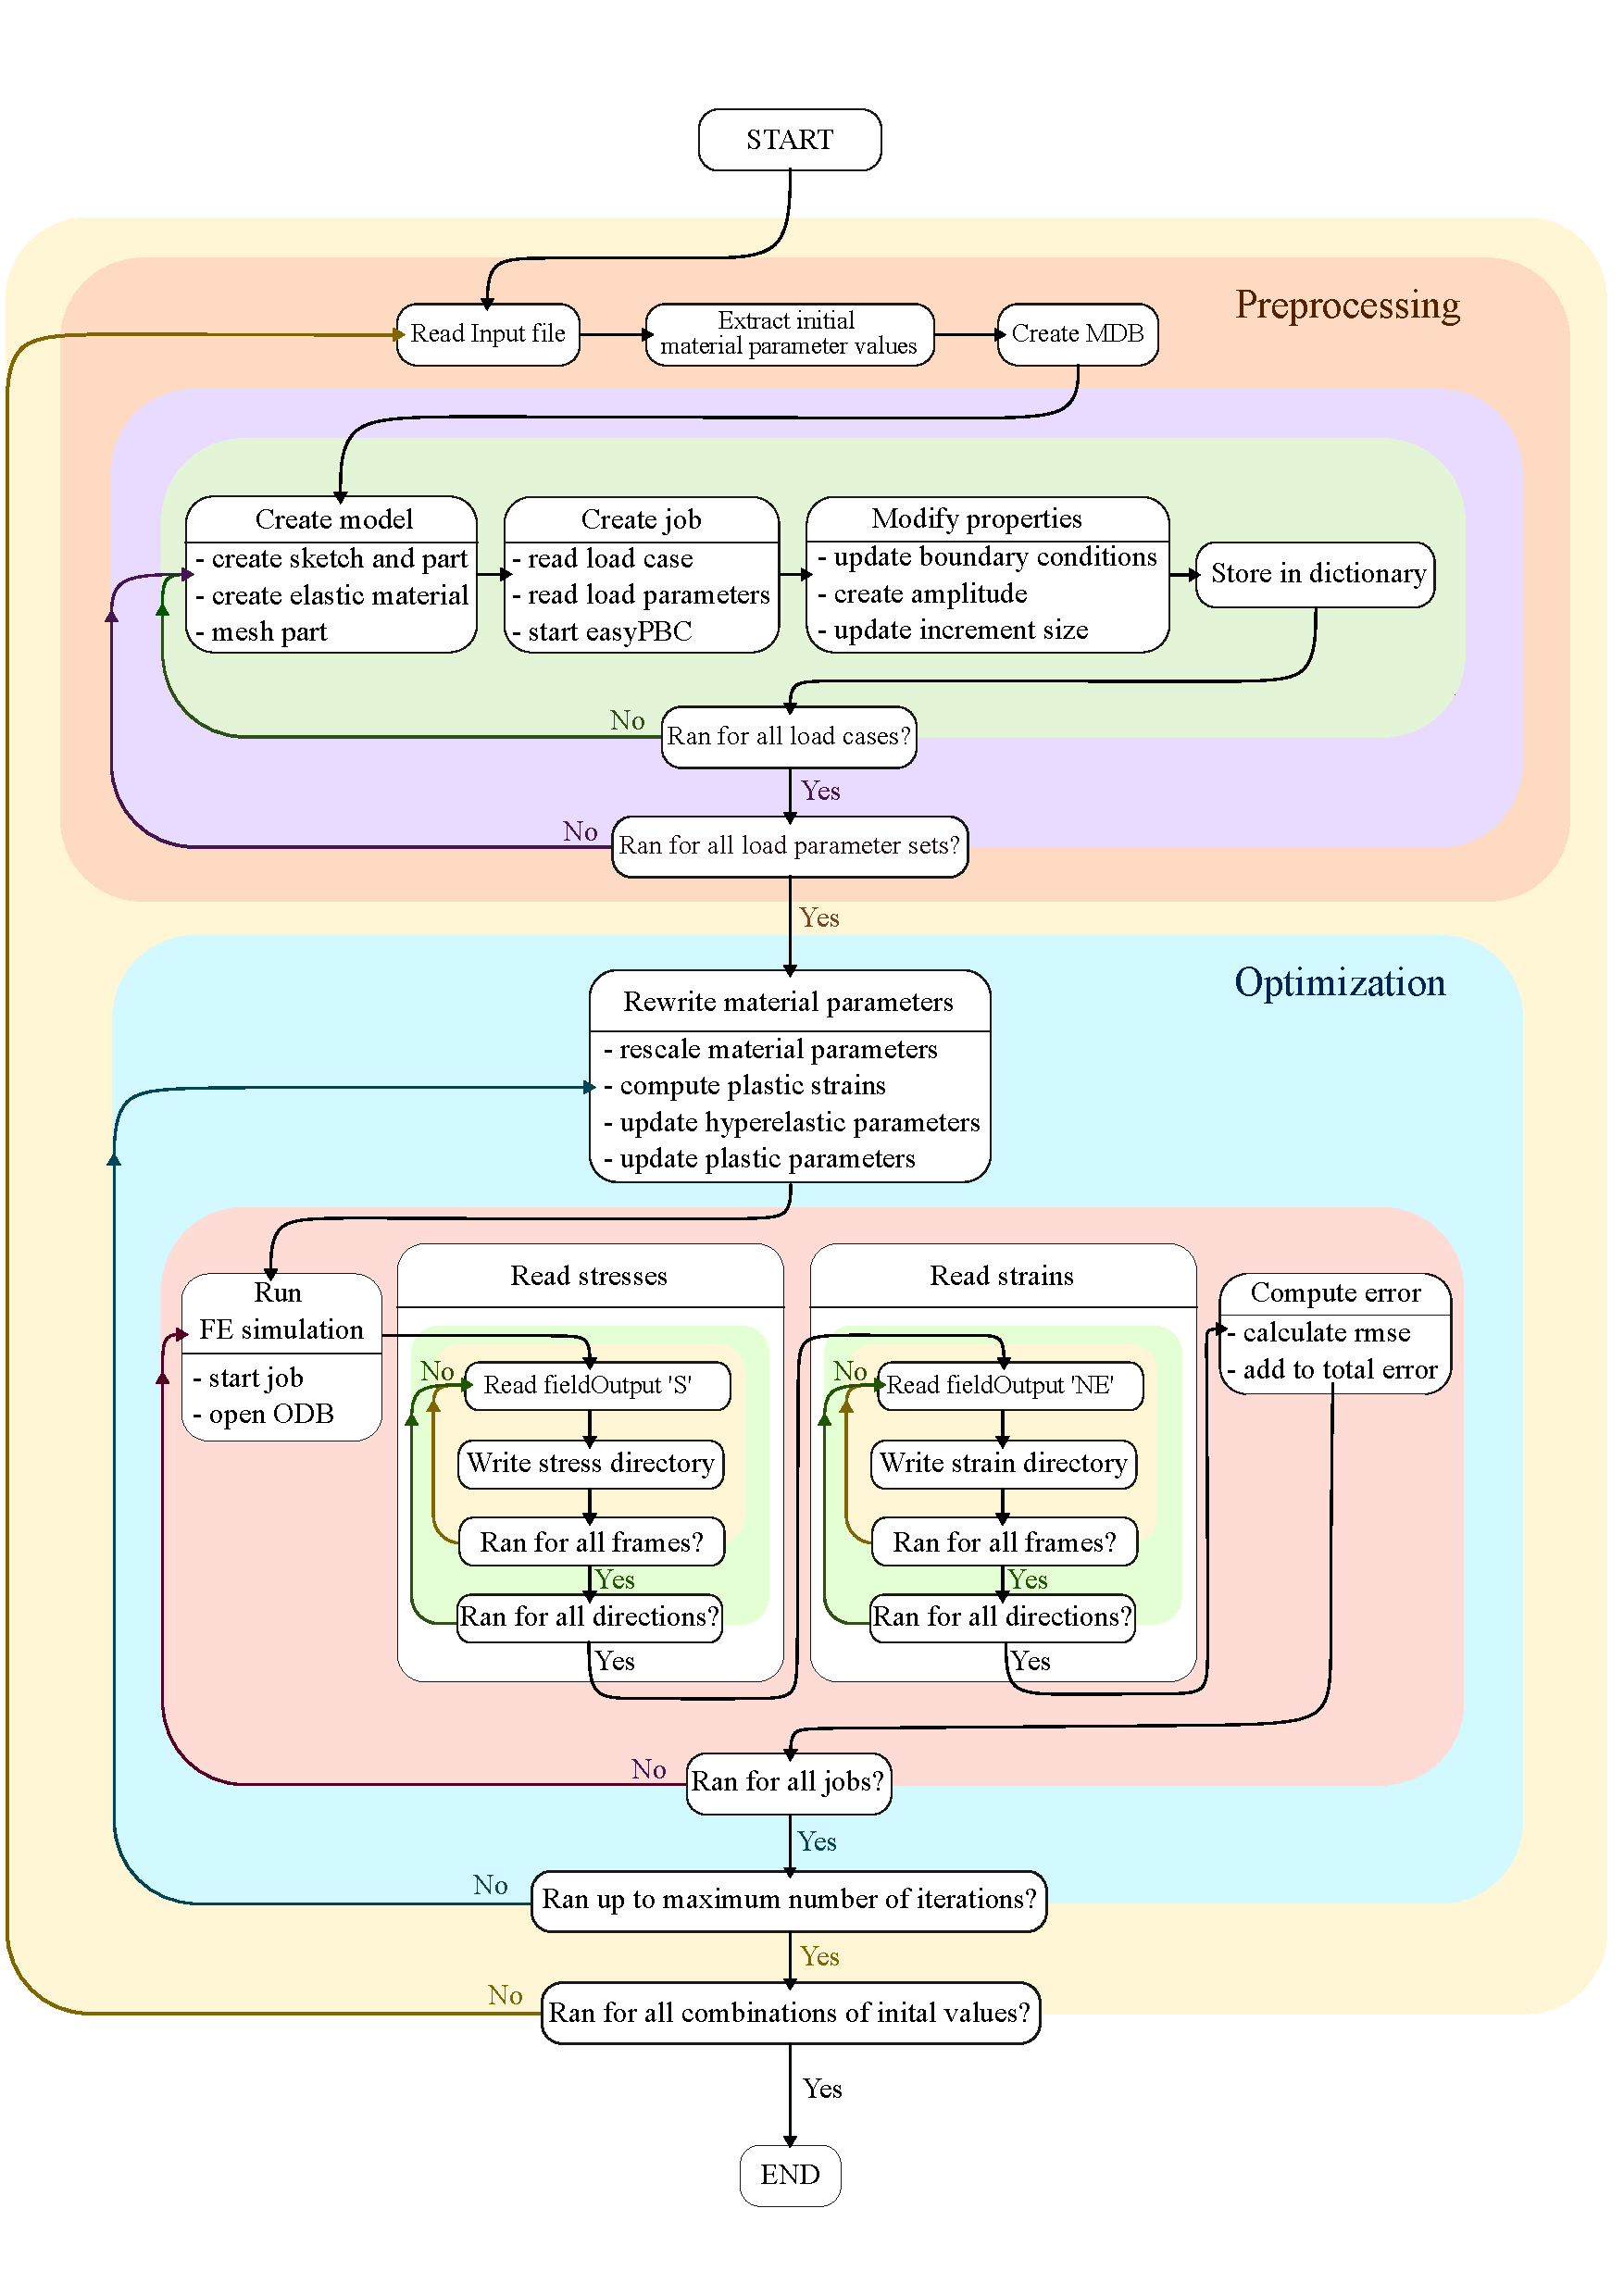
\includegraphics[width = 1.0\textwidth]{complete_flowchart_new.pdf}
    \caption{Flowchart code}
    \label{fig: flowchart}
\end{figure}

\begin{table}[h!]
\centering
\renewcommand{\arraystretch}{1.2}
\caption{Input parameters for SciPy minimize function}
\label{tab: minimizeFunctionInput}
\begin{tabular}{L{0.15\textwidth}|L{0.2\textwidth}C{0.12\textwidth}L{0.4\textwidth}}
\toprule
\textbf{Parameter} & \textbf{Content} & \textbf{Data format} & \textbf{Explanation} \\
\midrule
Objective function & Optimisation function & -- & Function whose scalar value should be minimized \\ \hline

Initial guess & Material parameters & array & Scaled initial values for the optimisation parameters \\\hline

\multirow{2}{0.15\textwidth}{Additional arguments}
 & Cube parameters & object & Model information from input file \\
 & Load parameters & dictionary & Load parameters from MD-simulations \\
 & Work directory & string & Path to store results \\
 & Evaluation counter & scalar & Counter for the performed function evaluations \\ \hline

method & Nelder-Mead & -- & Numerical algorithm \\\hline

bounds & Limits for material parameter & array & Upper and lower boundary values for every optimisation parameter \\\hline

maxiter & Number of iterations & scalar & Maximum number of iterations  as termination criterion\\
\bottomrule
\end{tabular}
\end{table}

In the following section, we describe the optimisation process. We start the process by calling the Scipy-minimize function. We pass this function various parameters, listed in \autoref{tab: minimizeFunctionInput}. The minimize function itself calls our self-written optimisation function, where the evaluation takes place. The initial guess stores an array with start values for all parameters that should be optimized. Additionally, we pass information about the models that we created in the preprocessing and the load parameters. We use all models created in the purple box for one optimisation call.
We start the process with the step \benennung{Rewrite material parameters} for all models. Since they all describe the same material, we write the same values for every model. For the minimization computation, optimisation parameters are scaled in the bounds from zero to one. To rewrite the values in the models, we have to rescale them first. Then we can use the rescaled parameters to compute the values for the plastic stress function with the formula for VOCE-hardening (\autoref{eq: voce}). In the following we remove the elastic material and substitute it with a hyperelastic material which is suitable for high non-linear deformations. Therefore, we have to convert the Young's modulus and the Poisson's ratio into the hyperelastic parameters $C_{10}$ and $D_1$ via the relations
\begin{gather}
    C_{10} = \frac{E}{4(1+ \nu)} \\
    D_1 = \frac{6(1-2\nu)}{E}.
\end{gather}

Now we can update all material values. In the next steps we handle the models successively. We start the job of the first model to perform the \name{Abaqus} analysis and open the resulting \acrshort{odb} in \benennung{Run FE-simulation}. With step \benennung{Read stresses} the evaluation begins. We do this by reading the 'FieldOutput' variable 'S' and write the data in a stress directory. Since we need stress-values at all steps defined by the amplitude, we read out every frame from the \acrshort{odb}. One frame corresponds with one step in the loading process. Additionally, we loop over all directions ($xx$, $yy$, $zz$, $xy$, $yz$, $xz$). The same procedure is done for the strain values in \benennung{Read strains}. Here it is important to read out the correct strain variable 'NE' (nominal strain). For hyperelastic materials, \name{Abaqus} uses the logarithmic strain ('LE') as standard value. Because of its logarithmic scaling, we cannot compare them to the reference data. Then we store all values for all frames and directions in a dictionary, similar as for the stresses. Now we have collected all required data to perform the step \benennung{Compute error}. We do this in the way described in \autoref{sec: errorCalculation}. For a better structure of the code this part is outsourced in a separate function. We call this function and pass the stress and strain directories as well as the corresponding load parameters. Then the computation runs and the function returns the \acrshort{rmse} for this job. Multiplied with its corresponding weights for its load case and load parameters we add this value to the total error value. Now we restart the red loop by starting the FE-simulation for the next job which is visualized in the red box in the flowchart. Once all the jobs are processed, and we computed the total error value, we return it to our minimization function. Through the internal Nelder-Mead algorithm the error is reduced and it returns the corresponding material parameters. Now one optimisation iteration is performed and it starts again. In the flowchart, the loop is visualized with the blue box. This process will run until our defined number of maximum iterations is reached or convergence is reached. When the changes in the error value are very small, the internal convergence criterion is reached and the algorithm stops.


\section{Storage of data} \label{sec: dataStorage}

To evaluate the optimization process at the end, parameter values need to be recorded during the preprocessing and the optimisation process. This is the only way to ensure that the values of all iterations are saved, since the variable values are rewritten in every new iteration. In the preprocessing, we extract the input file with the current initial value combination. All files created from \name{Abaqus} like the CAE, \acrshort{odb} and the job-files are stored in a subfolder. In the optimisation part, multiple functions are called after the step \benennung{Compute error} to store the current variable values. The material parameters for every iteration are stored. In addition, we store multiple interim results during the error calculation. For every job the weighted \acrshort{mse}s are stored for every iteration, so that the impact and evolution of every evaluated reactions can be understood. To track the impact of the applied weights, all \acrshort{rmse} values are stored individually and weighted. In addition, we store the total error, which is the sum of all weighted \acrshort{rmse}s of one iteration. Finally, we have one file each for the material parameters, \acrshort{mse}s, \acrshort{rmse}s, and the total errors. All these files are handled in the same way. After the computation of the total error, all files are opened and the variable values of the current iteration are stored in a new line. The stress and strains are stored in separate files for each iteration. We create for each job a subfolder, where its stress and strain values are stored. For one iteration, a file is created which contains the stress and strain dictionaries from the steps \benennung{Read stress} and \benennung{Read strain}. This leads to as many files as iterations were performed for every job. At the end of the optimisation process, we store the final message returned from the Scipy.minimize function. \name{Python} automatically sends a message where the cause of termination is stated. This message becomes important if the algorithm stops before the maximum number of iterations is reached. Then we can reproduce whether this happens because the convergence limit is reached or a numerical error occurred. The described procedure to store the data is done for every initial value combination separately.

TABELLE
MINIMIZE FUNCTION IN FLOWCHART INTEGRIEREN


% All data are stored in csv-format.

% - store results
% - welche results
% - material parameters for every iteration
% - rmse value for every iteration for every job (weighted and unweigthed)
% - total eror for every iteration
% - input file with inital value combination
% - abaqus model
% - stress and strain values for evaluated reactions for every iteration in sperate file
% - all in csv files
% - easy to handle 
% - kann gut direkt angeschaut werden und grobe einschätzung machen
% - leicht auszulesen
% - reference data
% - rmse message (message of scipy function) --> falls abbruch wg convergence error oder so 

